\section{Peak Calling}
Sequenziertes Genom/RNA/DNA aus dem Experiment = viele, kurze Reads

\hspace{10mm}$\rightarrow$ naiv: Jedes Nukleotid, dass von Reads bedeckt ist = Gebunden


\includegraphics[scale=0.5]{lectures/160415/pix/Peak1.png}

\hspace{15mm}$\rightarrow$ Problem: Viele FP, da kurze Reads mehrere Treffer haben können

\hspace{20mm}$\rightarrow$ Lösung: Cutoff für Anzahl der Reads auf Nukleotid

\hspace{25mm}$\rightarrow$ Problem: Manche Basen einfach zu binden = viele FP

So geht das nicht!
\newline\newline
Lösung:

\hspace{10mm} Enrichment: $log\frac{Expression}{Background}$

\hspace{23mm} naiv: Wenn Enrichtment $>$ Cutoff $\rightarrow$ Peak!

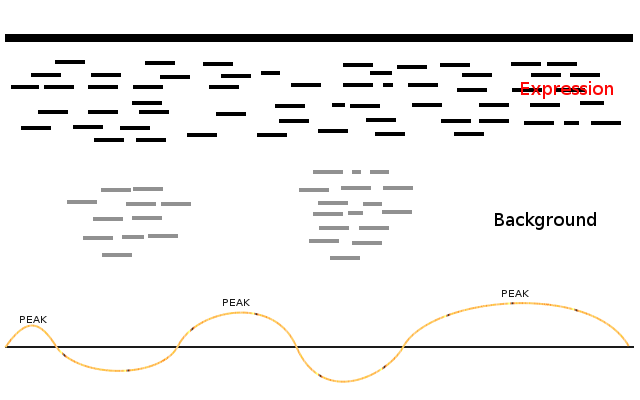
\includegraphics[scale=0.5]{lectures/160415/pix/Peak3.png}

\newpage
\subsection{MACS}
Model-based Analysis of ChIP-Seq (MACS)
\newline\newline
1. Einteilen des Genoms in Bins (Eimer)

\hspace{10mm} Window: 200 BP und Offset von 1/4 der window size

\hspace{10mm} In Bins werden Reads eingeordnet

2. Zählen der Fragmente pro Bin, +/- Strang

\hspace{10mm}$\rightarrow$ Poisson verteilt!
\newline

\hspace{10mm}$P(x>k,\lambda)=\sum_{i=k}^{\infty}P\lambda(i)=1-\sum_{i=0}^{k-1}P\lambda(i)=1-\sum_{n=0}^{k-1}\frac{\lambda^{n}}{n!}e^{-\lambda}$

$\lambda$=Mittelwert der read counts aus Background, k=read counts aus Experiment

\hspace{10mm}read count signifikant größer Mittelwert $\rightarrow$ Peak!

\hspace{10mm}Mittelwert kann abhängig von Menge der reads in Window sein:

\hspace{15mm} $\lambda$=max($\lambda$global, $\lambda$1000, $\lambda$5000, $\lambda$10000)

\hspace{15mm} $\rightarrow$ Window jeweils zentriert an Bin

3. p-Value Correction

\hspace{10mm} Holm-Bonferroni

\hspace{10mm} q-Value

4. Peakmerging

\hspace{10mm} Wenn Abstand zwischen Peaks $<$ Cutoff $\rightarrow$ Merge Peaks

\hspace{15mm} (bei MACS 2xWindowSize)
\\\\
\textbf{Wo sind die Bindungsstellen?}

Protein $\rightarrow$ RNA - \textbf{ChIP}: Regionen, mit denen das Protein assoziert ist

DNA $\rightarrow$ RNA - \textbf{ChIRP}: Match von RNA auf sequenzierter DNA

\hspace{47mm}Verfahren ähnlich zu CLIP

\hspace{47mm}$\rightarrow$RNA cross-linking(UV o. formalin)$\rightarrow$aufreinigen$\rightarrow$

\hspace{47mm}reverse cross-linking$\rightarrow$Read$\rightarrow$Match mit DNA

\hspace{47mm}(Chromatin isolation by RNA purification)

Protein $\rightarrow$ RNA - \textbf{RIP}: RNA zu cDNA, hybridisieren mit Chip

\hspace{47mm}$\rightarrow$RNA cross-linking(UV o. formalin)$\rightarrow$aufreinigen$\rightarrow$

\hspace{47mm}reverse cross-linking$\rightarrow$RNA in cDNA$\rightarrow$

\hspace{47mm}Hybridisierung auf Chip

\hspace{47mm}(RNA immunoprecipitation protocol)